% Anexos complementarios del Manual Técnico.
% Este archivo se incluye desde manual_tecnico.tex y conserva la numeración B.
% Las tablas son instrumentos de referencia y no representan datos productivos.

\subsubsection{Anexo B.1. Diagrama de arquitectura de referencia}
La Figura~\ref{fig:B_arquitectura} presenta la separación de responsabilidades documentada para el sistema. Angular concentra la interfaz; Python/FastAPI gestiona la lógica de negocio y los servicios; PostgreSQL conserva la información persistente.

\begin{figure}[H]
    \centering
    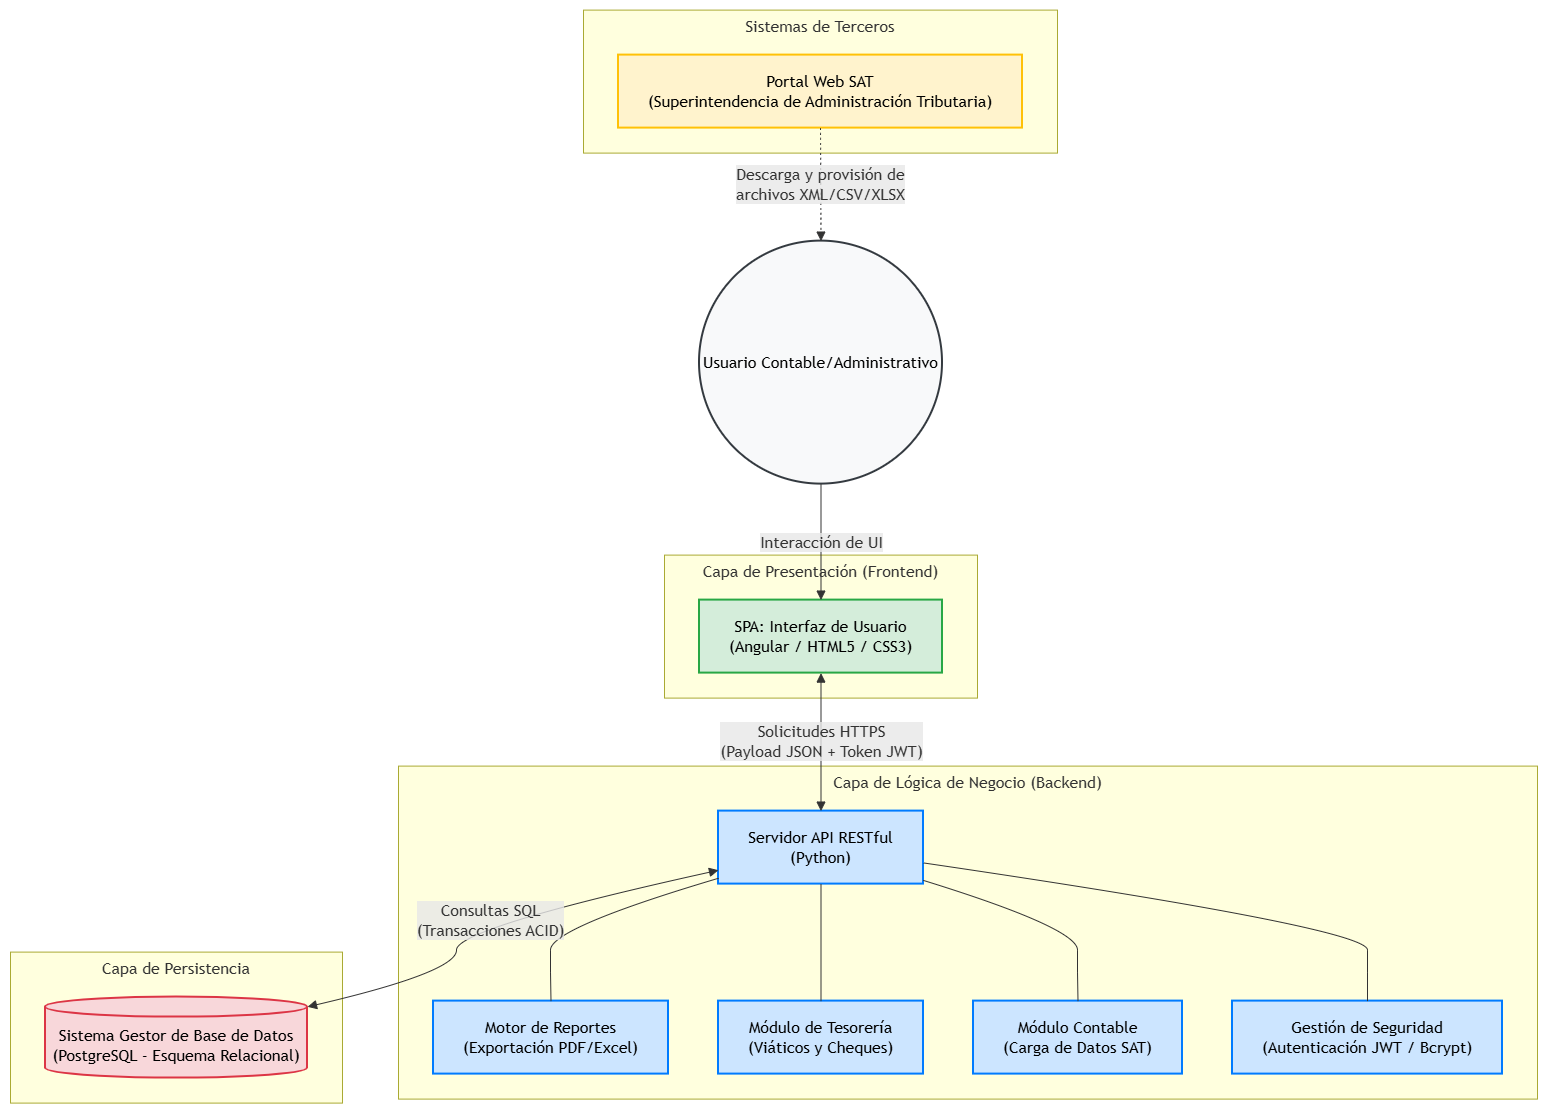
\includegraphics[width=0.92\textwidth]{imagenes/Arquitectura.png}
    \caption{Arquitectura de referencia del sistema}
    \label{fig:B_arquitectura}
\end{figure}

\subsubsection{Anexo B.2. Modelo de datos de referencia}
La Figura~\ref{fig:B_modelo_datos} presenta el modelo de datos utilizado como referencia para relacionar los módulos del sistema con PostgreSQL. Antes de aplicar cambios en producción, el responsable técnico debe validar la versión vigente del esquema y ejecutar un respaldo.

\begin{figure}[H]
    \centering
    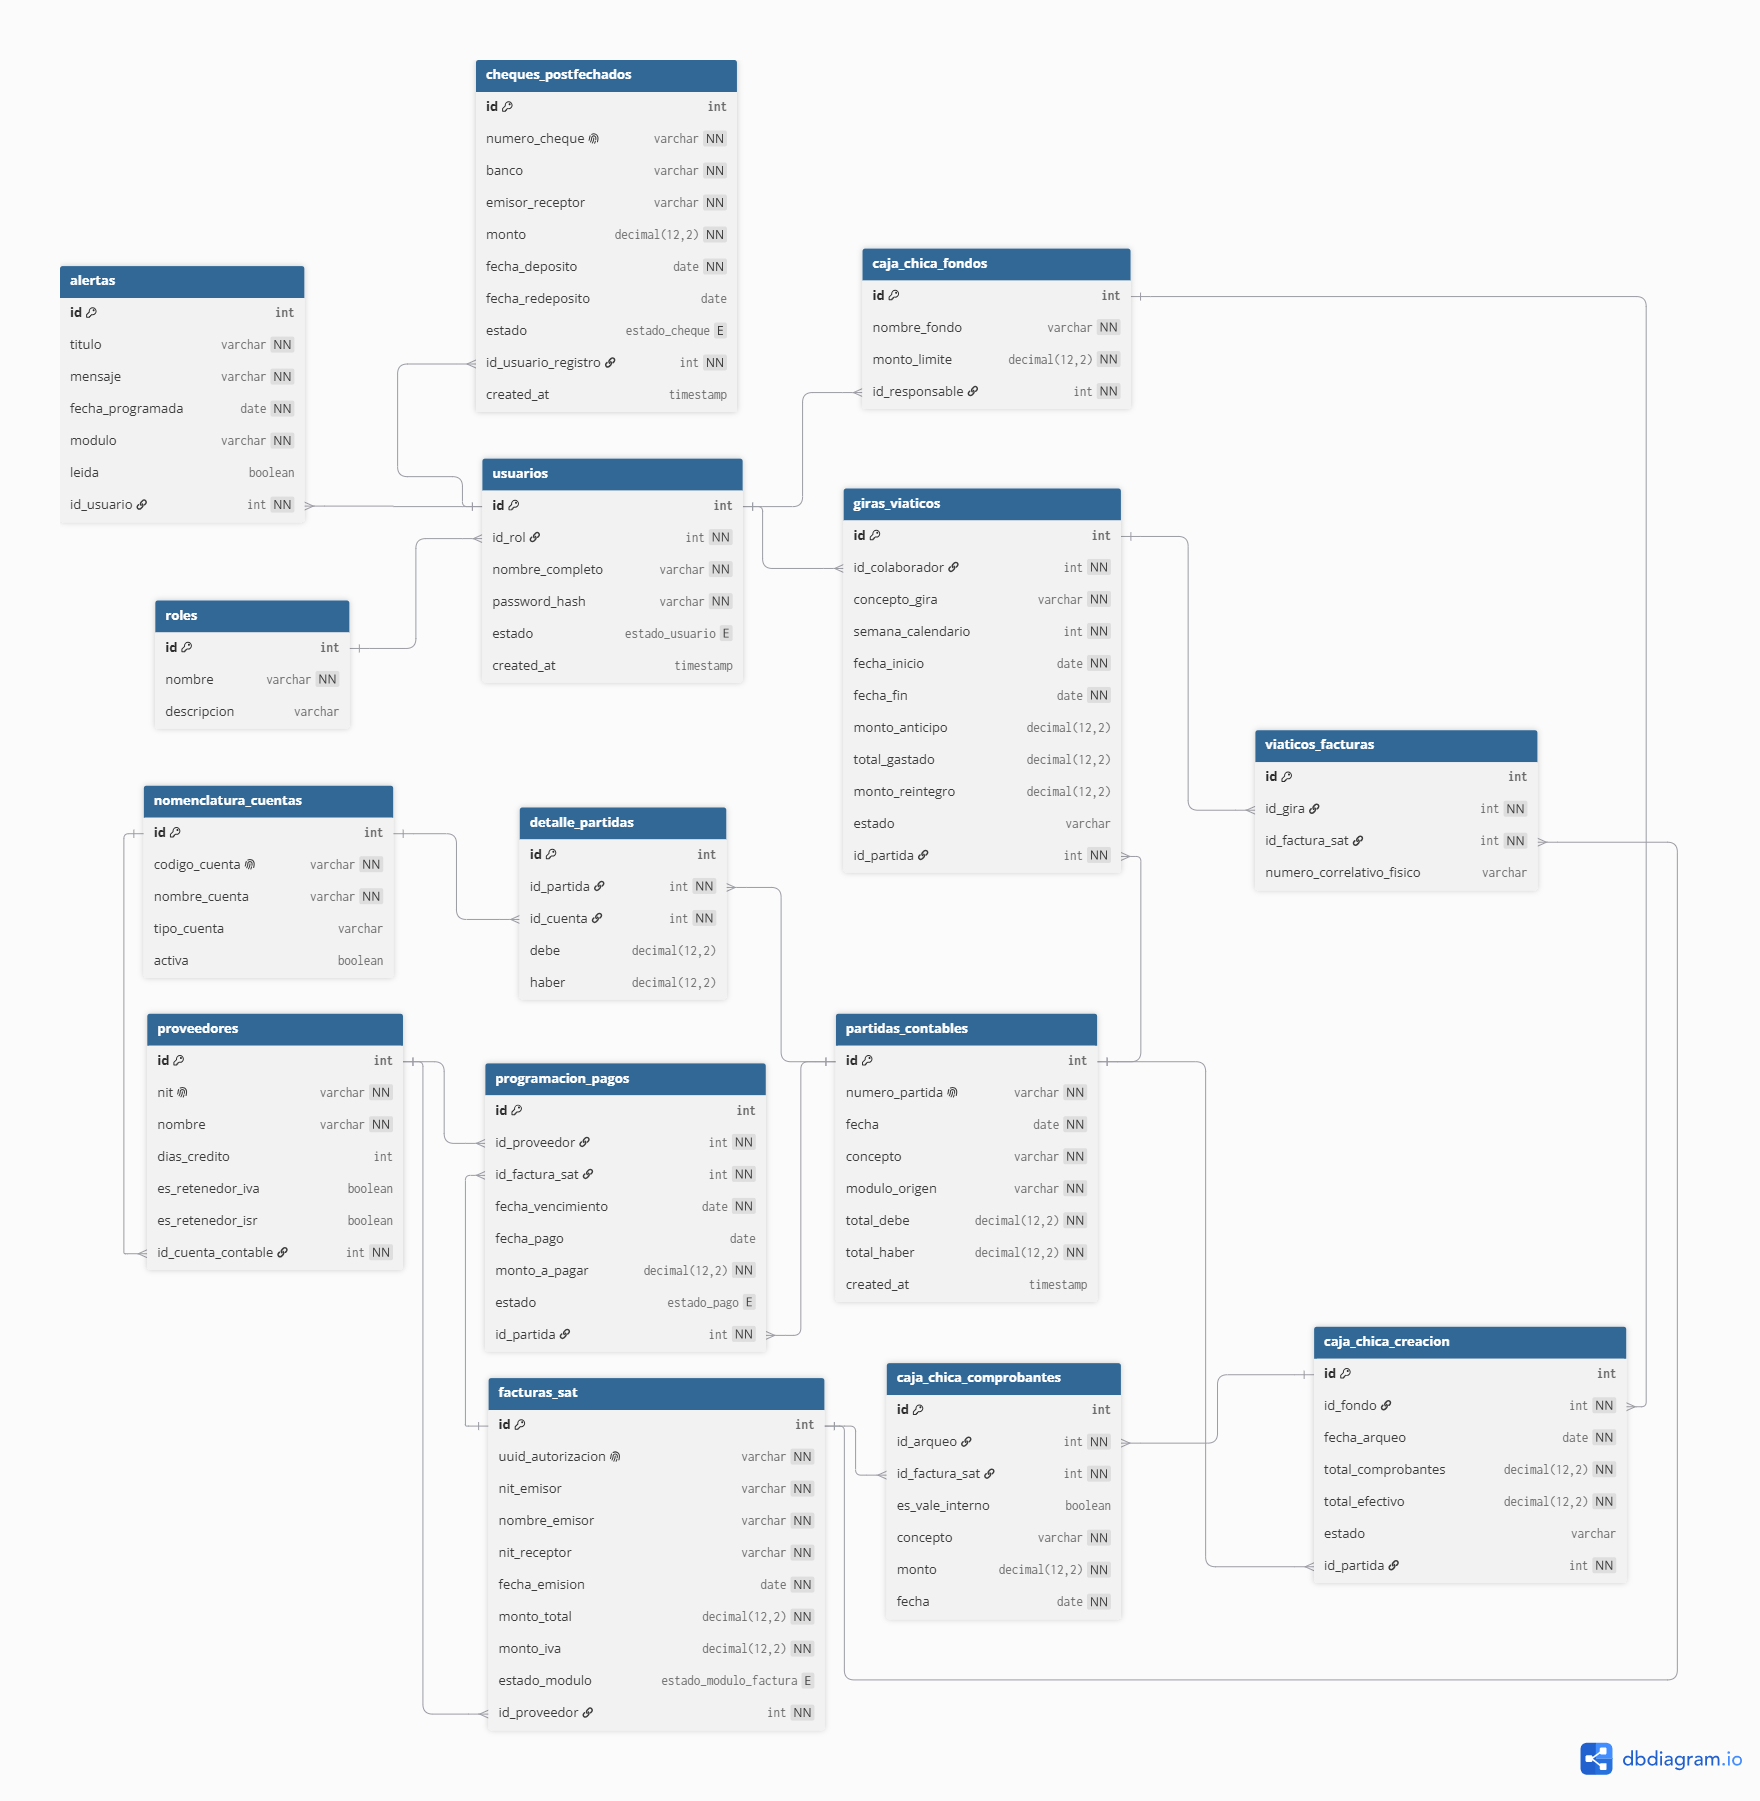
\includegraphics[width=0.95\textwidth]{imagenes/diagramabd.png}
    \caption{Modelo de datos de referencia en PostgreSQL}
    \label{fig:B_modelo_datos}
\end{figure}

\subsubsection{Anexo B.3. Matriz de trazabilidad técnica}
La Tabla~\ref{tab:B_trazabilidad_tecnica} relaciona los requerimientos funcionales documentados con los módulos, la capa principal involucrada y la evidencia disponible en la tesis.

\begin{longtable}{p{1.5cm}p{4.0cm}p{3.1cm}p{3.0cm}p{2.0cm}}
\caption{Matriz de trazabilidad técnica}\label{tab:B_trazabilidad_tecnica}\\
\toprule
\textbf{Req.} & \textbf{Funcionalidad} & \textbf{Módulo} & \textbf{Capa principal} & \textbf{Evidencia}\\
\midrule
REQ001 & Autenticación y acceso & Login & Angular/Python & Caso de uso y pantalla\\
REQ002 & Consulta de facturas FEL/SAT & Facturas FEL/SAT & Python/PostgreSQL & Caso de uso y pantalla\\
REQ003 & Registro de cheques posfechados & Cheques & Angular/Python & Caso de uso y pantalla\\
REQ004 & Registro y resumen de Caja chica & Caja chica & Angular/PostgreSQL & Caso de uso y pantalla\\
REQ005 & Liquidación y reintegro de Viáticos & Viáticos & Python/PostgreSQL & Caso de uso y pantalla\\
REQ006 & Asignación de facturas & Asignación & Angular/Python & Caso de uso y pantalla\\
REQ007 & Registro y cartera de proveedores & Proveedores & Python/PostgreSQL & Caso de uso y pantalla\\
REQ008 & Registro de nomenclatura contable & Nomenclatura & PostgreSQL/Python & Caso de uso y pantalla\\
REQ009 & Consulta de reportes & Reportes & Angular/Python & Caso de uso y pantalla\\
\bottomrule
\end{longtable}

\subsubsection{Anexo B.4. Lista de verificación de despliegue}
La siguiente lista debe completarse antes de habilitar una versión en un ambiente distinto al desarrollo. El responsable técnico debe conservar la evidencia de cada verificación.

\begin{longtable}{p{0.9cm}p{8.5cm}p{3.0cm}}
\caption{Lista de verificación de despliegue técnico}\label{tab:B_checklist_despliegue}\\
\toprule
\textbf{No.} & \textbf{Verificación} & \textbf{Estado}\\
\midrule
1 & Se confirmó la versión de Angular que será publicada. & \rule{2.5cm}{0.4pt}\\
2 & Se verificó la versión de Python y las dependencias del backend. & \rule{2.5cm}{0.4pt}\\
3 & Se configuraron las variables de entorno sin incluir secretos en el código. & \rule{2.5cm}{0.4pt}\\
4 & Se validó la conexión con PostgreSQL del ambiente destino. & \rule{2.5cm}{0.4pt}\\
5 & Se ejecutaron migraciones o cambios de esquema previamente revisados. & \rule{2.5cm}{0.4pt}\\
6 & Se realizó un respaldo antes de modificar la base de datos. & \rule{2.5cm}{0.4pt}\\
7 & Se verificó autenticación y permisos de los perfiles autorizados. & \rule{2.5cm}{0.4pt}\\
8 & Se ejecutaron pruebas de FEL/SAT, Cheques, Caja chica y Viáticos. & \rule{2.5cm}{0.4pt}\\
9 & Se revisaron logs y respuesta de los servicios después del despliegue. & \rule{2.5cm}{0.4pt}\\
\bottomrule
\end{longtable}

\subsubsection{Anexo B.5. Registro de respaldo y recuperación}
El registro siguiente permite documentar las pruebas de respaldo y recuperación de PostgreSQL. Debe completarse con información real de cada ejecución y conservarse según las políticas institucionales.

\begin{longtable}{p{2.3cm}p{3.0cm}p{3.0cm}p{3.0cm}p{2.0cm}}
\caption{Registro de respaldo y recuperación}\label{tab:B_registro_respaldo}\\
\toprule
\textbf{Fecha} & \textbf{Tipo de respaldo} & \textbf{Ambiente} & \textbf{Resultado de restauración} & \textbf{Responsable}\\
\midrule
 & Completo / incremental & Desarrollo / pruebas / producción & Pendiente de prueba & \\
 & Completo / incremental & Desarrollo / pruebas / producción & Pendiente de prueba & \\
 & Completo / incremental & Desarrollo / pruebas / producción & Pendiente de prueba & \\
\bottomrule
\end{longtable}

\subsubsection{Anexo B.6. Registro de mantenimiento}
Las actividades de mantenimiento deben registrar la fecha, la versión revisada, los cambios realizados y el resultado de las pruebas. No deben anotarse contraseñas, tokens ni credenciales dentro de este documento.

\begin{longtable}{p{2.3cm}p{3.2cm}p{5.2cm}p{2.0cm}}
\caption{Registro de mantenimiento técnico}\label{tab:B_registro_mantenimiento}\\
\toprule
\textbf{Fecha} & \textbf{Componente} & \textbf{Actividad realizada} & \textbf{Resultado}\\
\midrule
 & Angular & Actualización o revisión de interfaz y pruebas de navegación. & \\
 & Python/FastAPI & Revisión de dependencias, servicios y mensajes de error. & \\
 & PostgreSQL & Revisión de respaldo, espacio, permisos e integridad. & \\
 & Integración & Prueba de comunicación entre frontend, backend y base de datos. & \\
\bottomrule
\end{longtable}
